\section{Simulation}
Die beiden Steuerungsarten wurden mit Plecs und Matlab simuliert um genauer analysieren zu können, wie sich diese verhalten. 
a\\
a\\
a\\
a\\
a\\
a\\


\subsubsection{Einphasige Phasenanschnittsteuerung}
Für die einphasigen Phasenanschnittsteuerung mit Plecs ist der Zwei-Puls-Generator von sehr grosser Bedeutung. 



\subsection{Simulation mit Matlab}
Um die einphasige Plecs-Simulationen der Phasenanschnitt- und Schwingungspaketsteuerung zu verifizieren wurde parallel zur Plecs-Simulation das gleiche Verfahren mit Matlab vorgenommen. Mit Hilfe dieser Überprüfung konnte davon ausgegangen werden, dass die die Überlegungen sowie der Aufbau der Plec-Simulation stimmt und somit ohne weiteres bedenken das dreiphasige Vorgehen der zwei Verfahren mit Plecs verwirklichen kann. Im folgenden Kapitel wird nun aufgezeigt, welche Überlegungen man bei den Matlabfunktionen vorgenommen hat und wie die Ergebnisse zustande kamen. Ausserdem werden die Resultate der Matlab-Simulationen mit den Plecs-Simulationen verglichen und dokumentiert.

Die ersten Funktionen, die man simulierte, waren periodische Sinusfunktionen im Zeitbereich mit verschiedenen Phasenanschnitten. Die Periodenlänge definierte man dabei auf 2$\pi$ und die Amplitude des Sinus auf ± 1. Der Winkel des Phasenanschnittes wurde mit verschieden, geläufigen Werte wie zum Beispiel $30^\circ$, $45^\circ$, $60^\circ$, $90^\circ$ oder $120^\circ$ betrachtet. In den Abbildungen \ref{fig:Einganssignal 60} erkennt man die Sinusfunktionen mit einem Phasenanschnitt von links \ref{fig:Einganssignal 60} $60^\circ$ und rechts \ref{fig:Einganssignal 90} $90^\circ$. Weitere Funktionen mit den anderen Winkeln sind im Anhang ersichtlich.
 

\begin{figure}[h]
	\centering
	\subfloat[][]{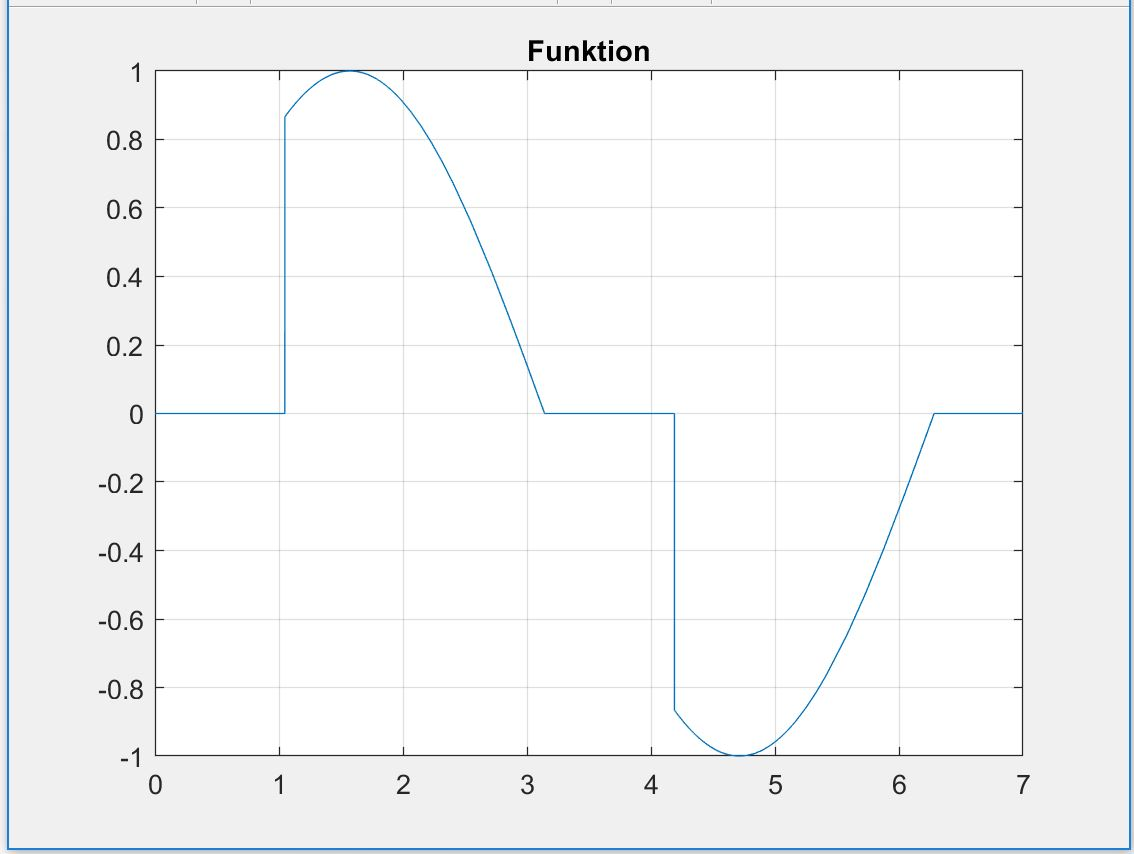
\includegraphics[width=0.47\linewidth]{eingangssignal_60.png}\label{fig:Einganssignal 60}}\qquad
	\subfloat[][]{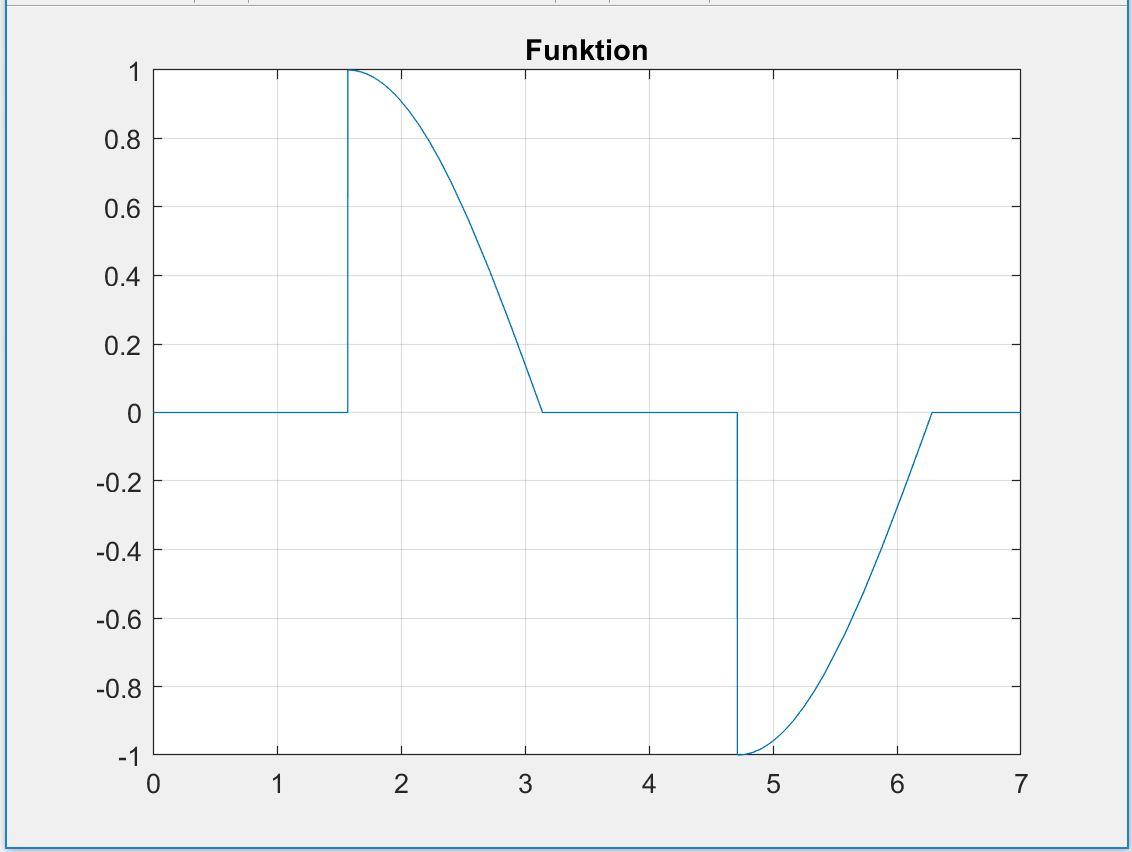
\includegraphics[width=0.47\linewidth]{eingangssignal_90.png}\label{fig:Einganssignal 90}}
	\caption{Einganssignal mit Phasenanschnitt a) $60^\circ$ (b) $90^\circ$}
	\label{fig:eingangssignal}
\end{figure} 


Als nächstes nahm man die Zerlegung der Funktion in verschiedene Frequenzanteile vor. Dies wird auch als Fourier-Analyse bezeichnet. Man erhielte somit mit der Berechnung der Fourier-Koeffizienten $a\textsubscript{0}$,$b\textsubscript{n}$ und $a\textsubscript{n}$ eine Phasen- und Amplitudenspektrum. Die Darstellung im Zeitbereich beziehungsweise im Frequenzbereich sind äquivalent, sie enthalten also die vollständige Information über die Funktionen. Im Spektrum benutzt man die vertikalen Linien, um die Frequenzkomponenten anzugeben. Die x-Achse ist somit die Frequenz der Frequenzkomponente und die y-Achse gibt die Länge der Komponente an. In den untenstehenden Grafiken \ref{fig:Amplituden- und Phasenspektrum} erkennt man das Amplituden- und Phasenspektrum des in Abbildung \ref{fig:eingangssignal} dargestellten Signale.

\begin{figure}[h]
	\centering
	\subfloat[][]{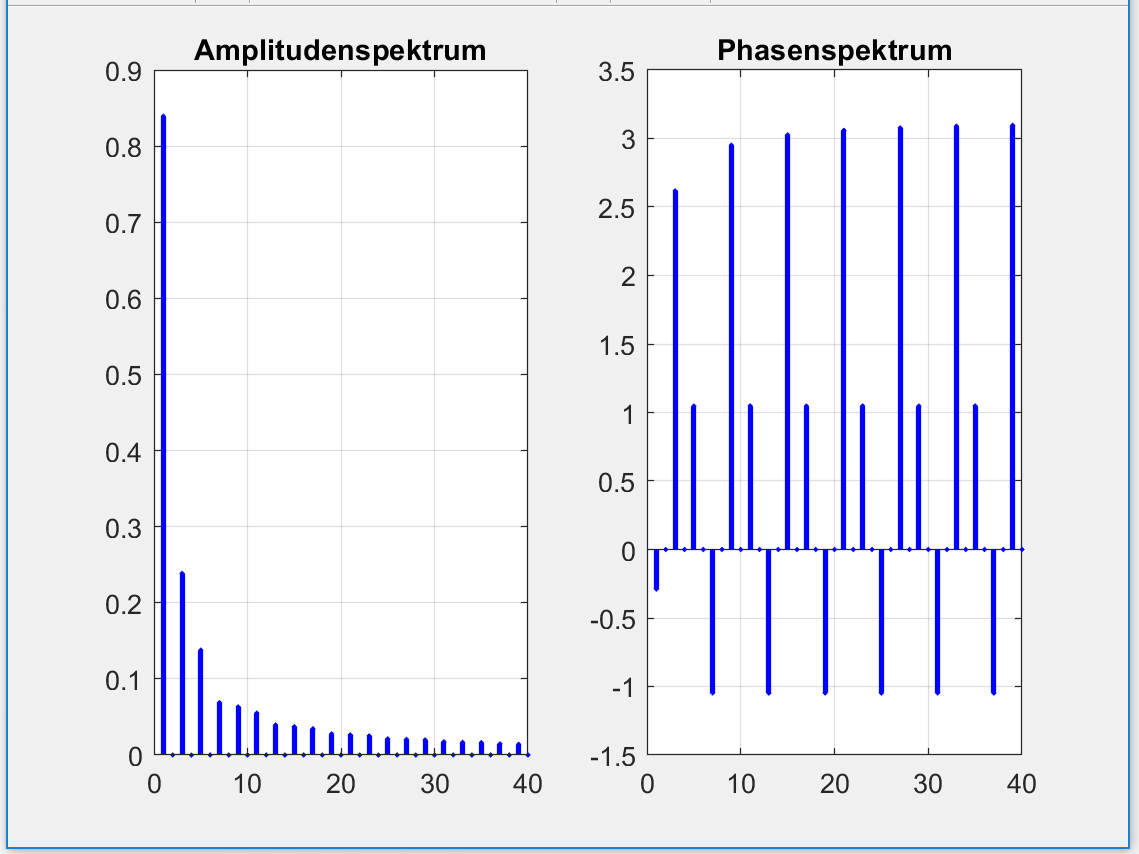
\includegraphics[width=0.47\linewidth]{A_PH_60.png}\label{fig:Amplituden- und Phasenspektrum 60}}\qquad
	\subfloat[][]{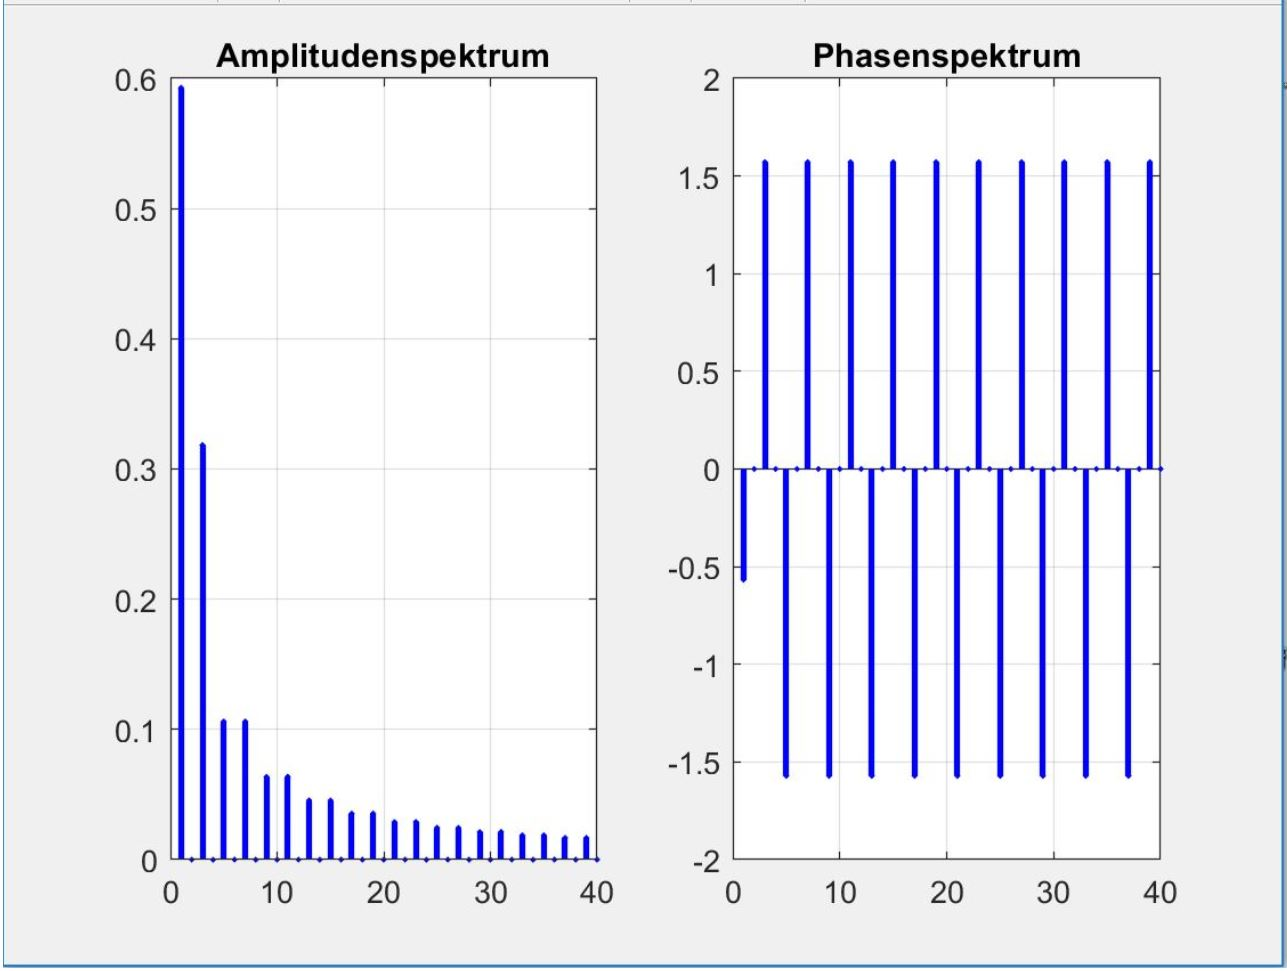
\includegraphics[width=0.47\linewidth]{A_PH_90.png}\label{fig:Amplituden- und Phasenspektrum 90}}
	\caption{Amplituden- und Phasenspektrum (a) $60^\circ$ (b) $90^\circ$}
	\label{fig:Amplituden- und Phasenspektrum}
\end{figure} 

Zur Überprüfung der Berechnungen und der Darstellung des Amplituden- und Phasenspektrum, wurde mit diesen zwei Spektren das Eingangssignal rekonstruierte. Dieses Signal erkennt man auf der nächsten Abbildung \ref{fig:Rekonstruiertes Signal}. Es ist ersichtlich das die Rundung des Sinus nicht genau dem, des eigentlichen Signal entsprechen \ref{fig:eingangssignal}. Dies kommt davon, dass man die Funktion in «nur» 40 Frequenzanteile unterteilt hat. Würde man eine grössere Anzahl Anteile verwenden, so könnte das Rauschen noch mehr verkleinern werden. Da man jedoch nur einen ungefähren Vergleich der beiden Signale haben möchte, reicht diese Anzahl völlig aus. 

\begin{figure}[h]
	\centering
	\subfloat[][]{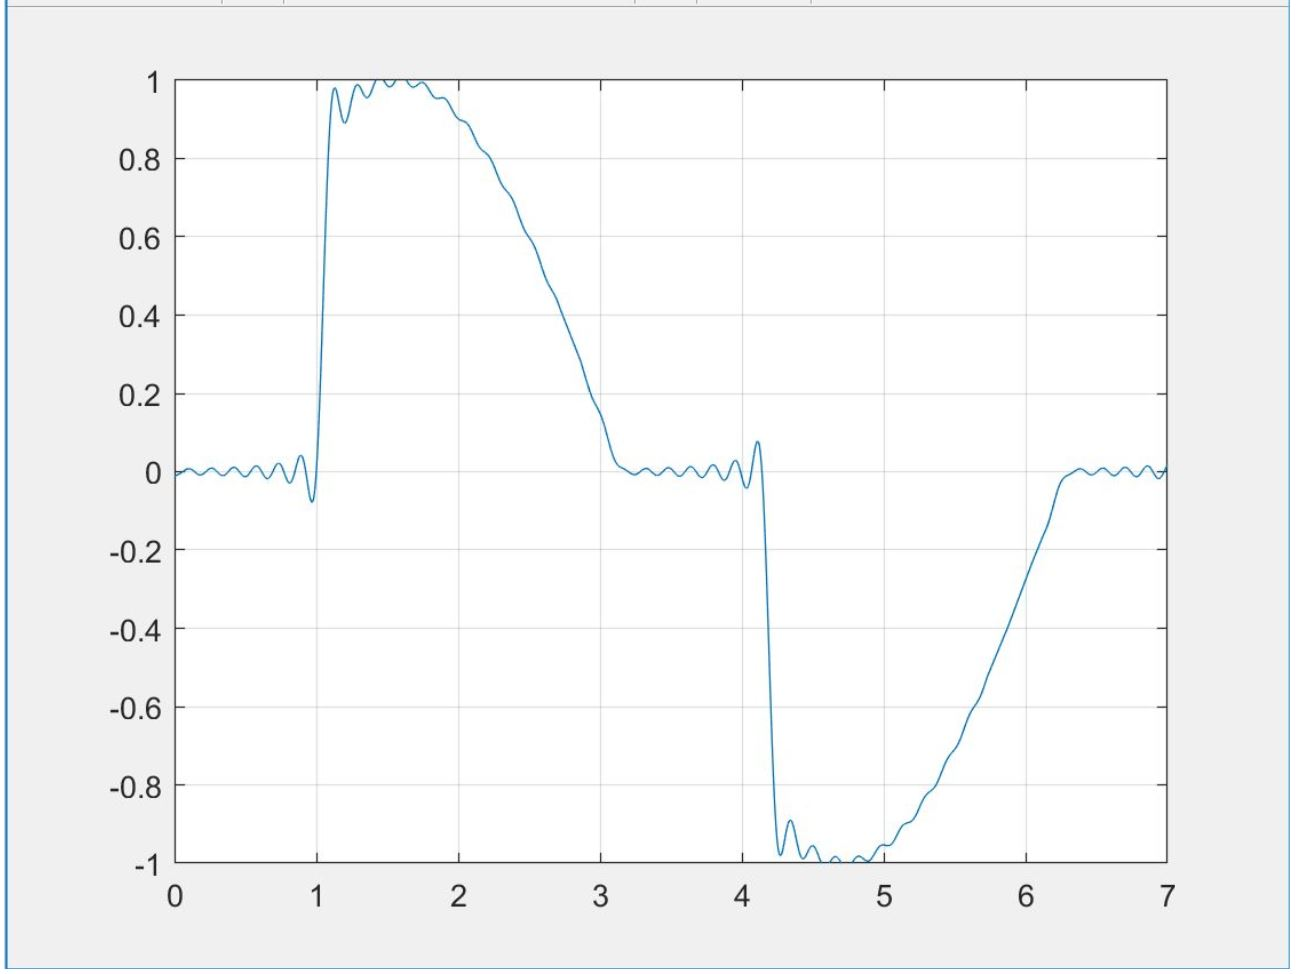
\includegraphics[width=0.47\linewidth]{re_eingangssignal_60.png}\label{fig:rekonstruiertes Signal 60}}\qquad
	\subfloat[][]{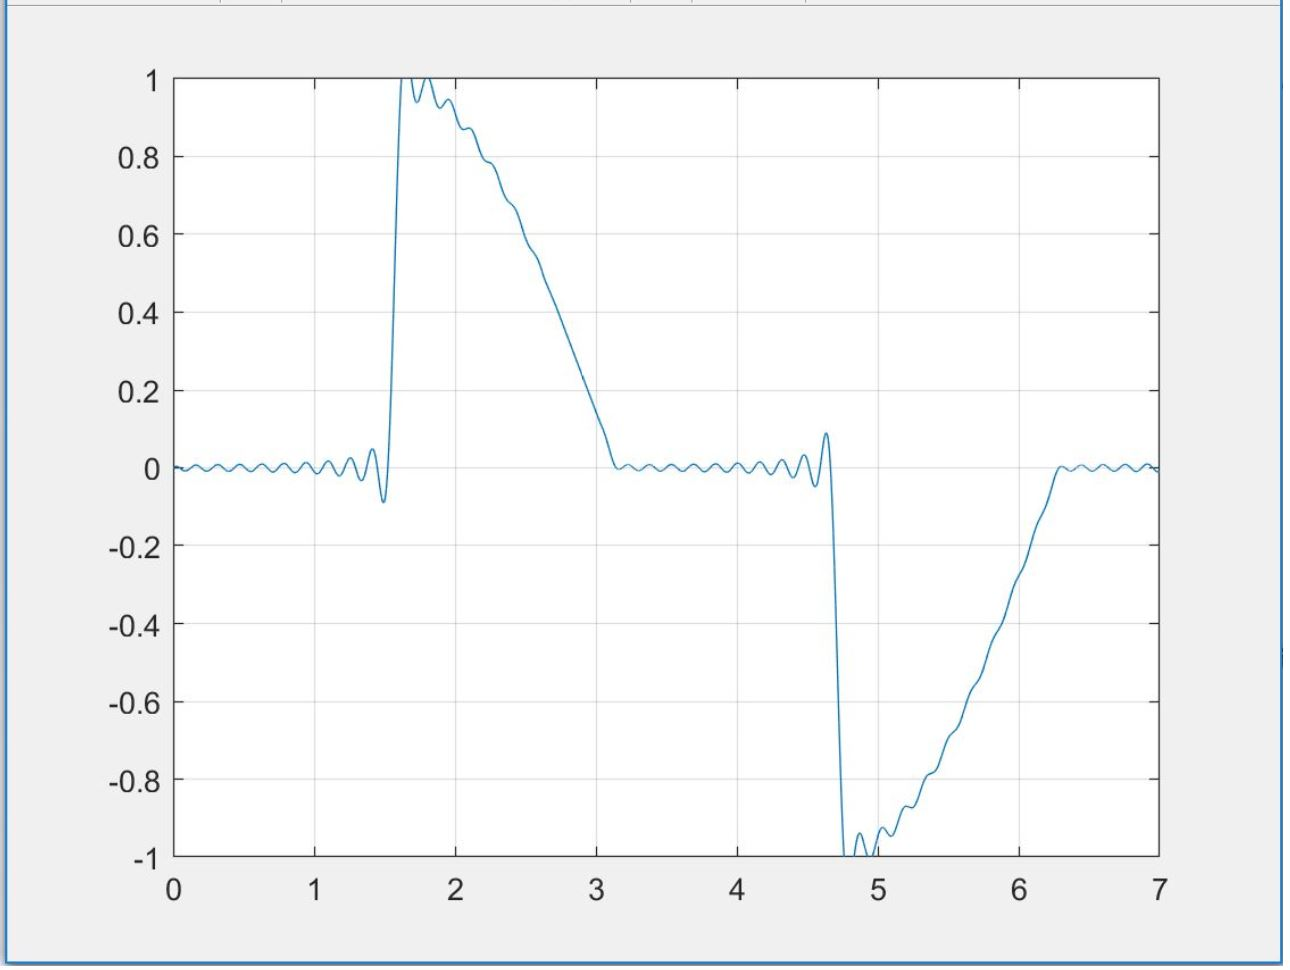
\includegraphics[width=0.47\linewidth]{re_einganssignal_90.png}\label{fig:rekonstruiertes Signal 90}}
	\caption{Rekonstruiertes Signal (a) $60^\circ$ (b) $90^\circ$}
	\label{fig:Rekonstruiertes Signal}
\end{figure} 


Nach dem man das Phasenanschnittsignal, das Amplituden- und Phasenspektrum, und das rekonstruierende Eingangssignal von Hand berechnet und geplottet wurde, überprüfte man mit Hilfe der FFT-Funktion (Fast Fourier Transform) von Matlab die Werte und die Grafiken. In der folgenden Abbildung \ref{fig:FFT mit Matlab} erkennt man die Plots bei einem Winkel von $60^\circ$. Bei dem Amplituden- und Phasenspektrum wurde die x-Achse so normiert, dass die Werte ein Vielfaches der Grundfrequenz von 50 Hz sind. So ist zum Beispiel der Wert bei 500 beim FTT zu vergleichen mit dem Wert bei 10 bei der Berechnung von Hand.

\begin{figure}[ht!]
	\centering
	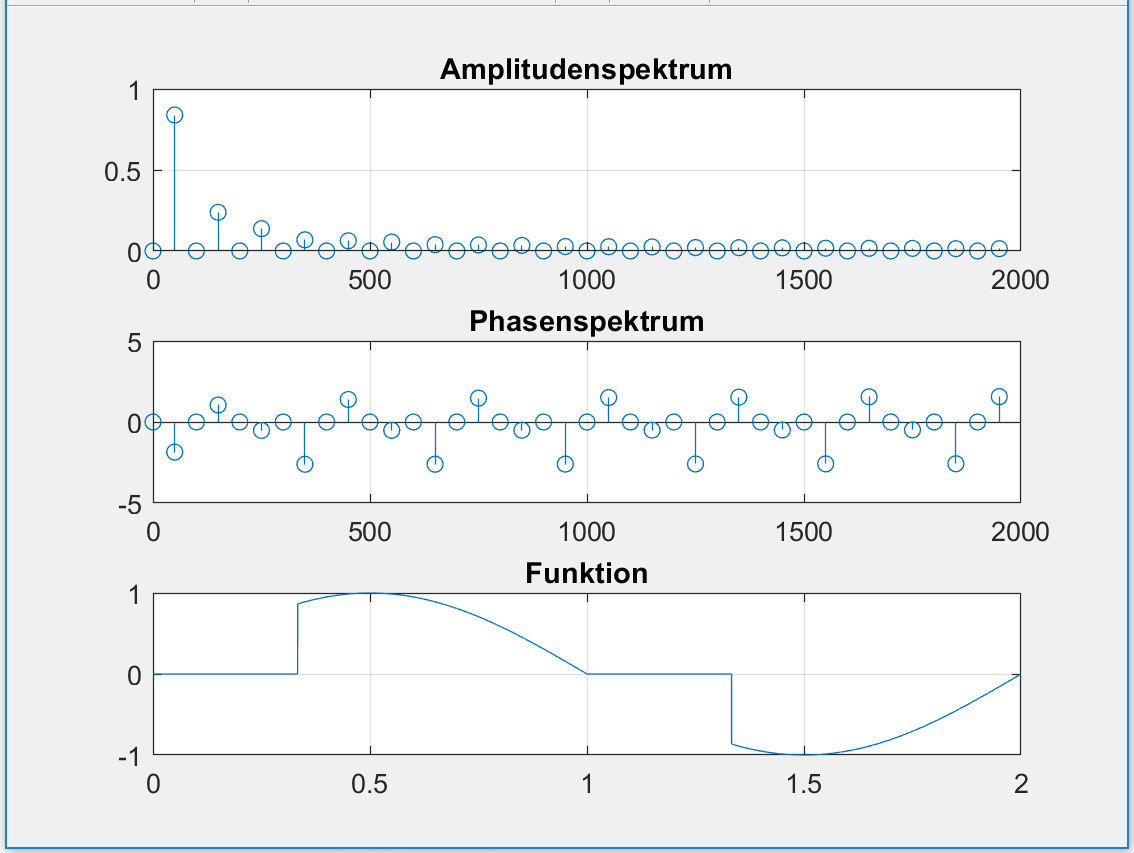
\includegraphics[scale=0.7]{FFT_mit_Matlab.png}	
	\caption{FFT mit Hilfe der Matlabfunktion}
	\label{fig:FFT mit Matlab}
\end{figure}

Bei der zweiten Funktion, die zu überprüfen und simulieren war, handelte es sich um eine Schwingungspaketsteuerungen. Die komplette Paketdauer beträgt bei den abgebildeten Funktionen 20 Halbwellen \ref{fig:Schwingungspaket Matlab}. Es wurden nun verschiedene Einschaltverfahren untersucht. In der Abbildung  erkennt man links \ref{fig:Schwingungspacket 0.5} einen duty cycle von 0.5, es sind dementsprechend immer 10 Halbwellen  ausgeschaltet und die anderen 10 eingeschaltet. Auf der rechten Seite \ref{fig:Schwingungspacket 0.8} beträgt der Wert des duty cycle 0.8. Es sind also zuerst 4 Halbwellen ausgeschaltet und die restlichen 16 Halbwellen werden angesteuert. Für einen sinnvollen Vergleich mit der Plec-Simulation wurden 5 Schwingungspakete untersucht. Die Leistungen der rechten Funktion ist somit 1/2 und die der linken 8/10 so gross wie die der normalen Netzspannung.

\begin{figure}[h]
	\centering
	\subfloat[][]{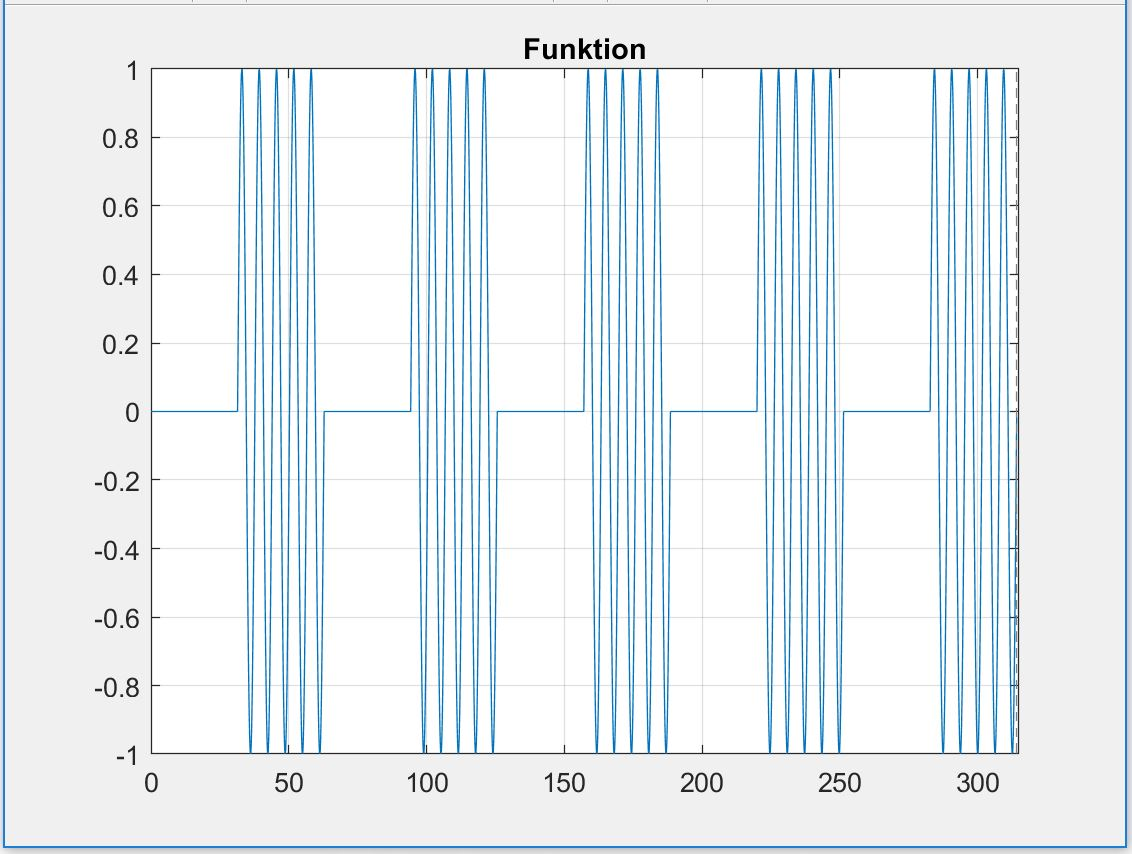
\includegraphics[width=0.45\linewidth]{Schwingungspaket_0_5.png}\label{fig:Schwingungspacket 0.5}}\qquad
	\subfloat[][]{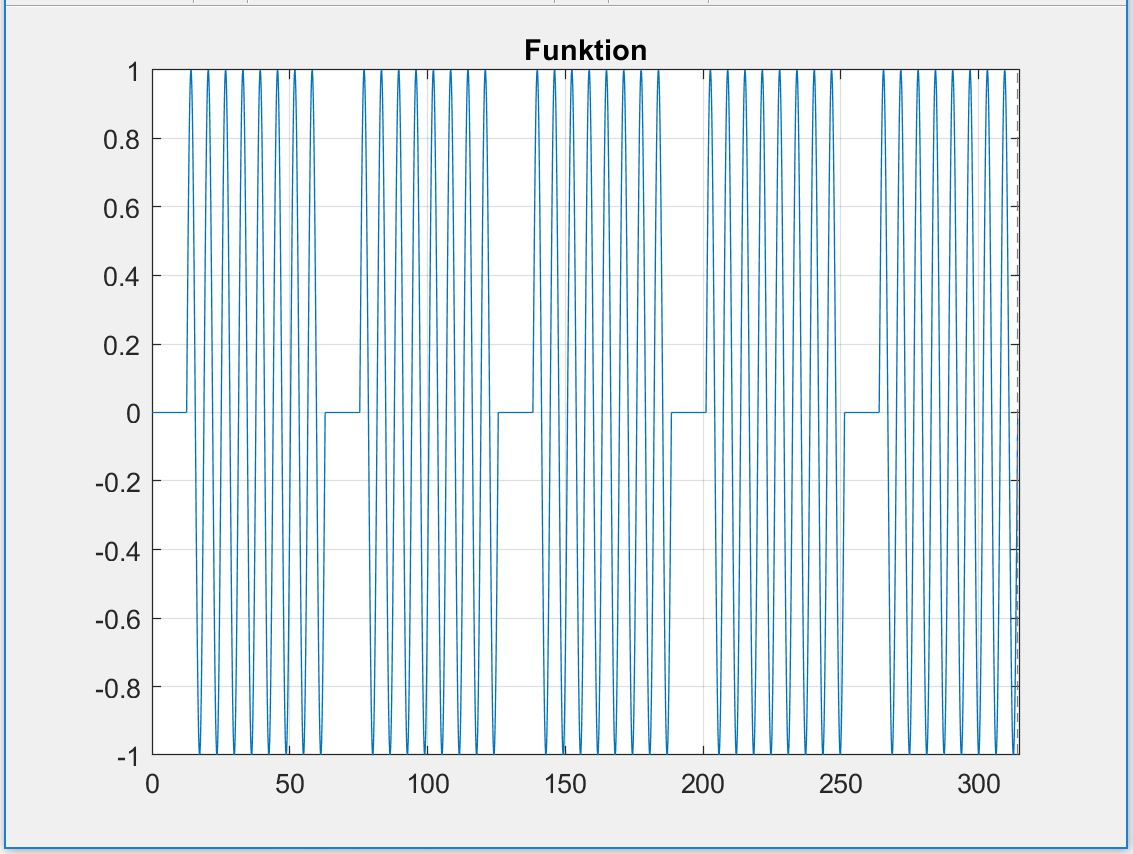
\includegraphics[width=0.45\linewidth]{Schwingungspaket_0_8.png}\label{fig:Schwingungspacket 0.8}}
	\caption{Schwingungspaket mit einem duty cycle von (a) 0.5 (b) 0.8}
	\label{fig:Schwingungspaket Matlab}
\end{figure} 

Um auch hier die Plecs-Simulation zu überprüfen, stellte man das absolute lineare Spektrum dar \ref{fig:Schwingungspaketspektrum Matlab}. Die unteren  Abbildungen zeigen die Spektren, links mit einem duty cycle von 0.5 \ref{fig:Schwingungspacketspektrum 0.5} und rechts mit einem von 0.8 \ref{fig:Schwingungspacketspektrum 0.8}. Interessant sind da vor allem die Subharmonischen Schwingungen, welche sich unterhalb der Grundfrequenz von 50 Hz befinden. Sie sind jeweils auf der linken Seite der Grafiken veranschaulicht. Damit man einen besseren Überblick über die Oberschwingungen erhält, wurde das Spektrum bis auf 1000 Hz erweitert. Dies ist auf der rechten Seite des jeweiligen Bildes ersichtlich. Vergleicht man die zwei Bilder erkennt man, dass je höher der duty cycle ist desto höher ist der Peak-Wert bei der Grundfrequenz 50 Hz. 

\begin{figure}[h]
	\centering
	\subfloat[][]{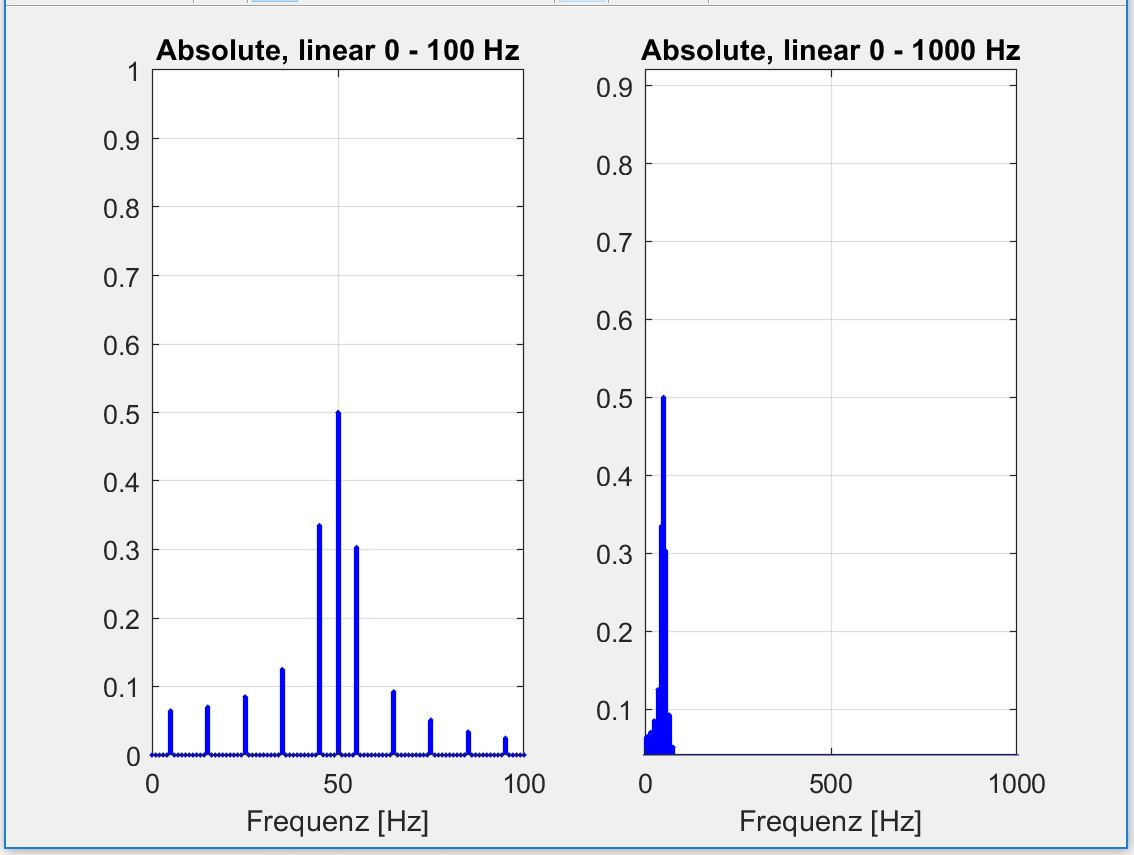
\includegraphics[width=0.45\linewidth]{Oberwellen_0_5.png}\label{fig:Schwingungspacketspektrum 0.5}}\qquad
	\subfloat[][]{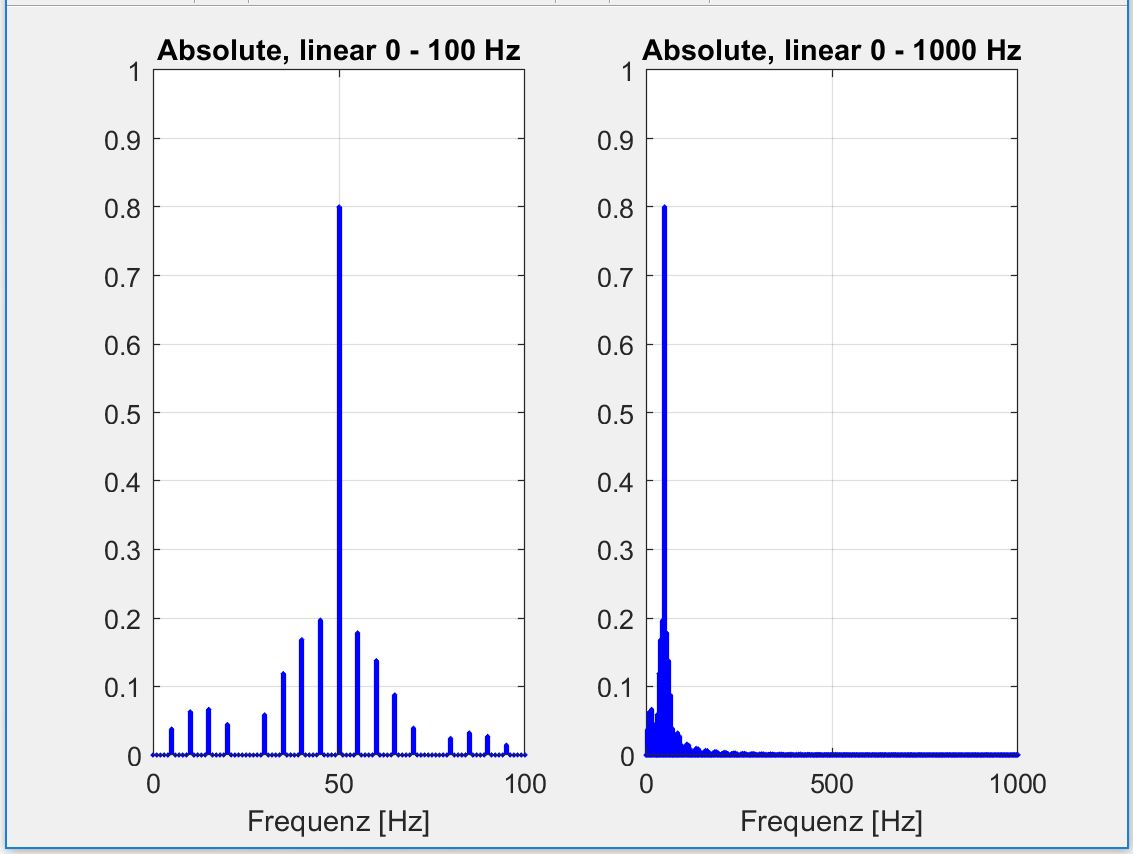
\includegraphics[width=0.45\linewidth]{Oberwellen_0_8.png}\label{fig:Schwingungspacketspektrum 0.8}}
	\caption{Lineares absolutes Spektrum mit einem duty cycle von (a) 0.5 (b) 0.8}
	\label{fig:Schwingungspaketspektrum Matlab}
\end{figure}

Schlussendlich untersuchte man noch den absoluten Logarithmus der beiden Funktionen. Die ist in der Abbildung \ref{fig:absolut_logaritmic_matlab} zu erkennen. Die y-Achse zeigt das Verhältnis der Spannungen an, dies wird immer in Dezibel angegeben. Bei der x-Achse handelt es sich um die Frequenz welche man untersucht hat. Auch hier wurde der absolute Logarithmus mit den zwei duty cycle 0.5 \ref{fig:absolut_logarithmic_0.5} und 0.8\ref{fig:absolut_logarithmic_0.8} untersucht.


\begin{figure}[h]
	\centering
	\subfloat[][]{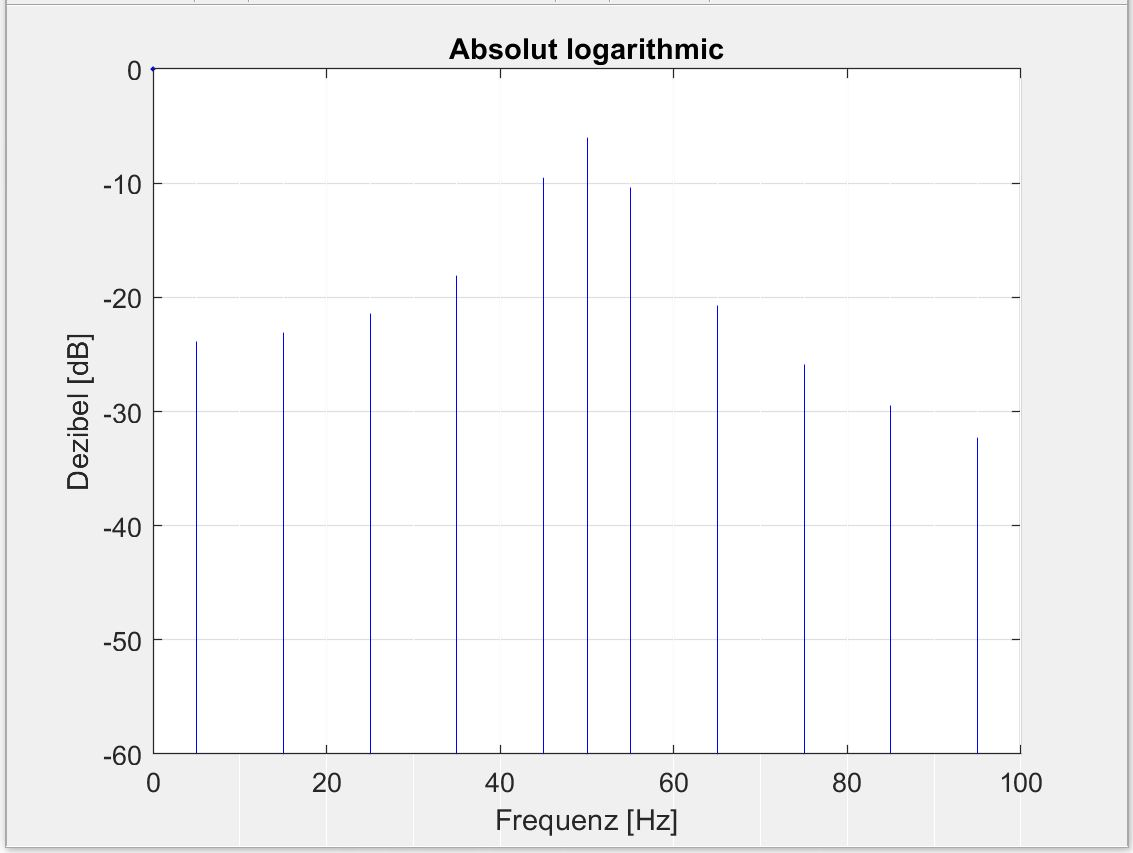
\includegraphics[width=0.45\linewidth]{absolut_logaritmic_0_5.png}\label{fig:absolut_logarithmic_0.5}}\qquad
	\subfloat[][]{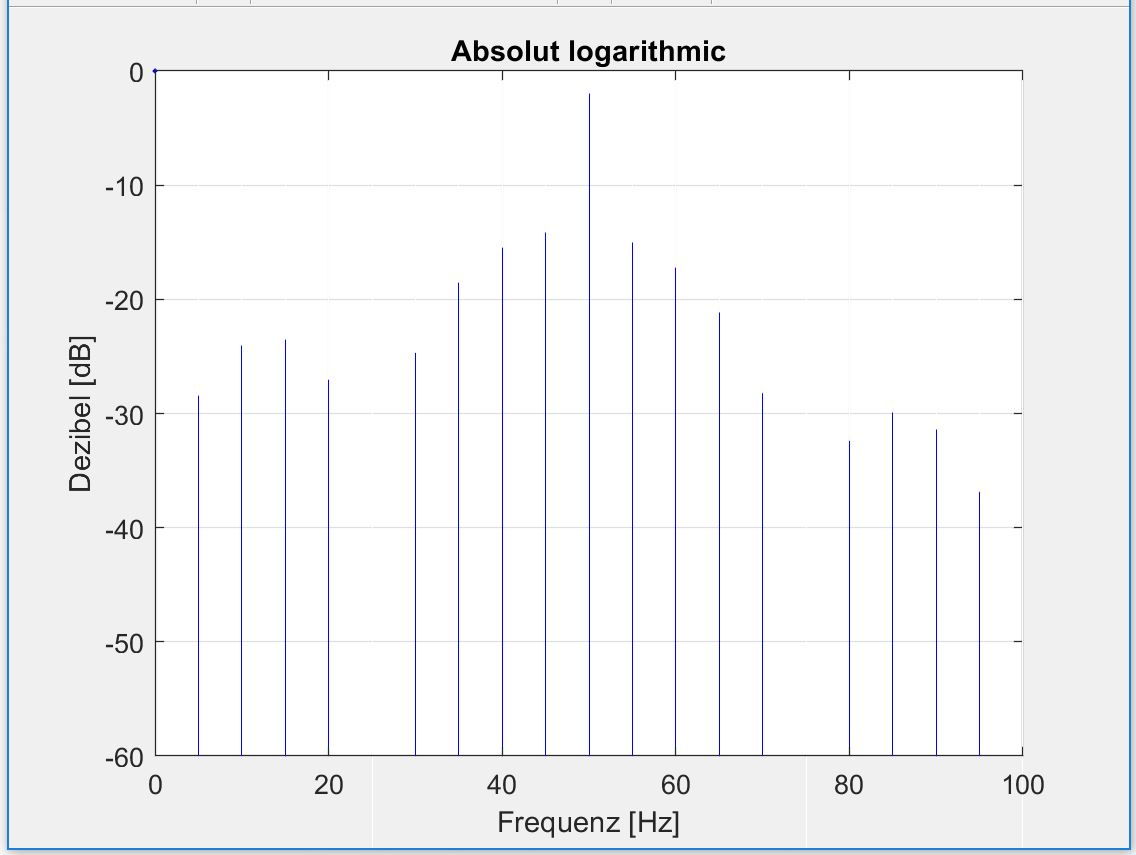
\includegraphics[width=0.45\linewidth]{absolut_logaritmic_0_8.png}\label{fig:absolut_logarithmic_0.8}}
	\caption{Lineares absolutes Spektrum mit einem duty cycle von (a) 0.5 (b) 0.8}
	\label{fig:absolut_logaritmic_matlab}
\end{figure}
\newpage
\subsection{Simulation mit Plecs}

Mit dem Simulationsprogramm Plecs konnte man alle gewünschten Ansteuerungen simulieren. Die einphasigen Simulationen der Phasenanschnitt- und der Schwingungspaketsteuerung wurden mit den Matlab-Funktionen verglichen und so auf ihre Richtigkeit überprüft. Nach dem man dies verifiziert hat, stellte man Verfahren für den dreiphasigen Phasenanschnitt- und Schwingungspaketsteuerung her. Ausserdem konstruierte man Kombinationen der beiden Verfahren im einphasigen und dreiphasigen System.\todo{alle Verfahren auflisten} Die Resultate sind auf den folgenden Seiten aufgezeigt.

\begin{figure}[h]
	\centering
	\subfloat[][]{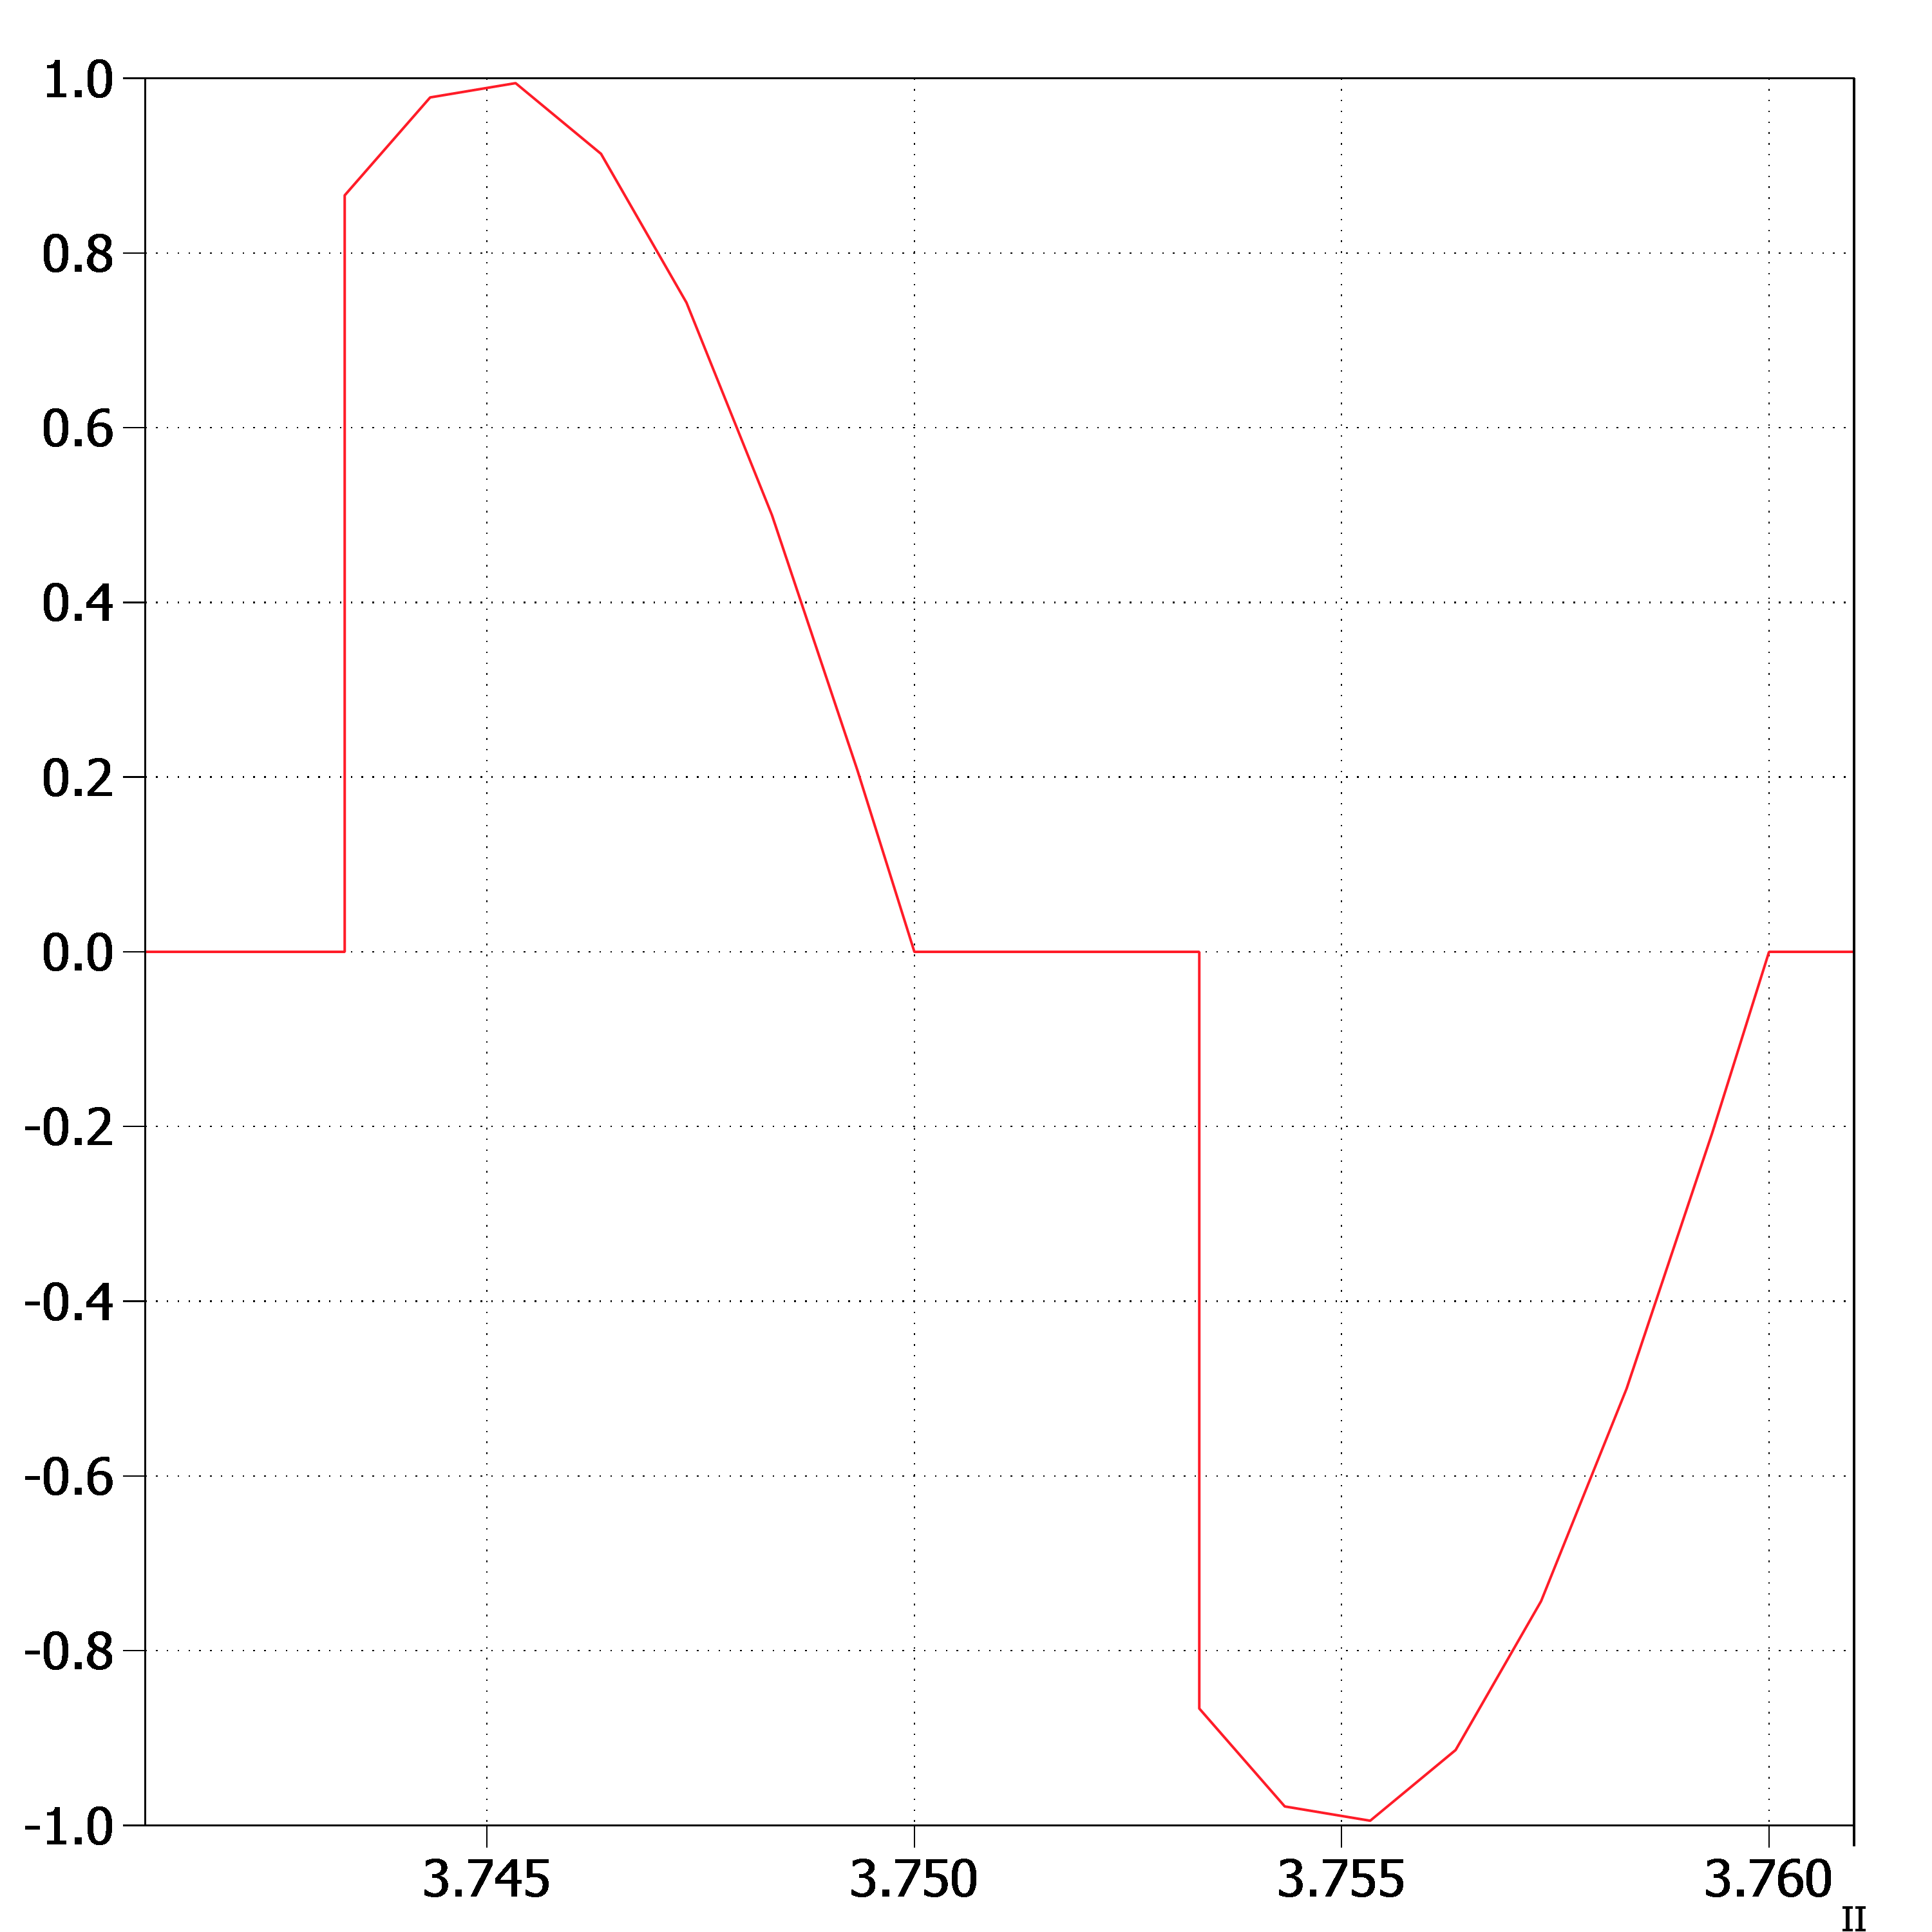
\includegraphics[width=0.45\linewidth]{plecs_phasenanschnitt_pi_3_funktion.png}\label{fig:plecs_eingangssignal_60}}\qquad
	\subfloat[][]{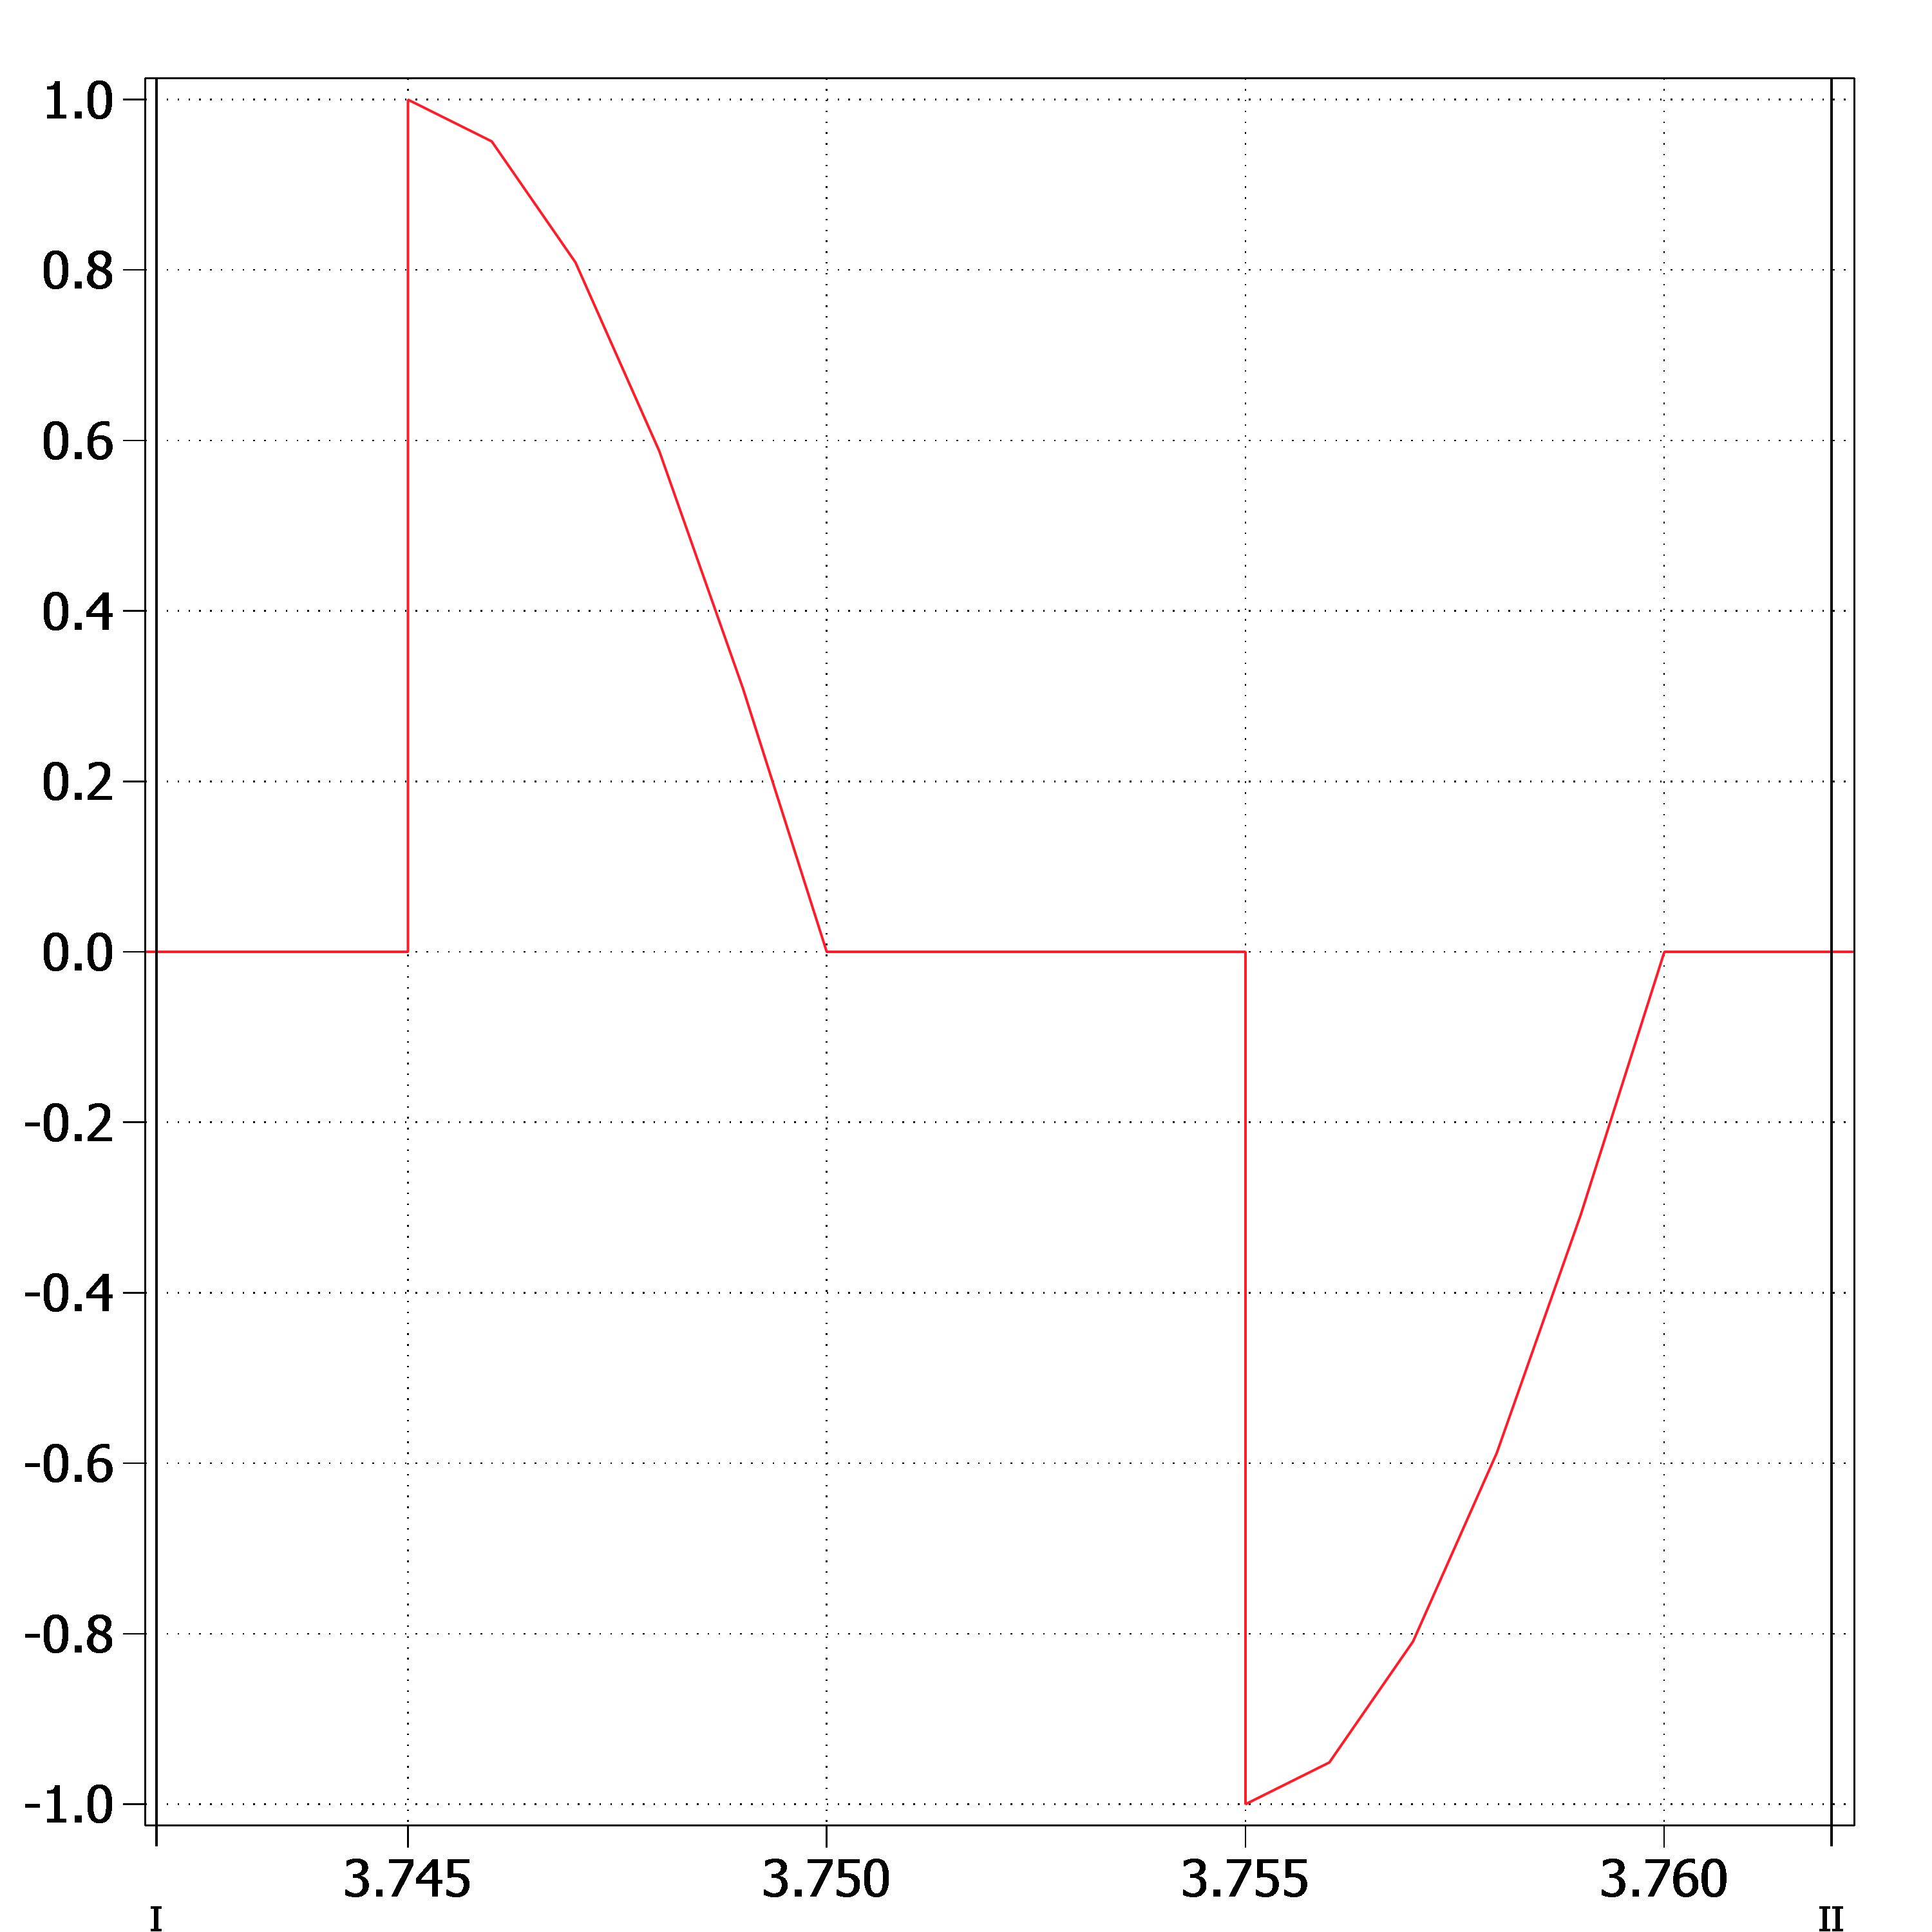
\includegraphics[width=0.45\linewidth]{plecs_phasenanschnitt_pi_2_funktion.png}\label{fig:plecs_eingangssignal_90}}
	\caption{Eingangssignal mit Phasenanschnitt (a) 60° (b) 90°}
	\label{fig:Eingangssignal simuliert mit Plecs}
\end{figure}




 


